\documentclass{article}
\usepackage[a4paper]{geometry}
\usepackage[utf8]{inputenc}
\usepackage[french]{babel}

\usepackage{graphicx}
\usepackage{courier}
\usepackage{listings}

\usepackage[svgnames]{xcolor}
\xdefinecolor{darkgreen}{named}{DarkGreen}

\lstdefinelanguage{lustre}{%
   columns=fullflexible,%
   basicstyle=\tt\footnotesize,
   % keywordstyle=\bfseries,
   commentstyle=\slshape,%
   keywords={%
     node,var,let,tel,returns,
     when,merge
   },%
   keywordstyle={\color{darkgreen}\sffamily},%
   morekeywords=[2]{%
     int, real, bool,
   },%
   keywordstyle=[2]{\color{blue}\ttfamily},%
   classoffset=2,%
   morekeywords=[3]{%
     storage, parameter, code %
   },%
   morekeywords=[3]{
     True,False
   },
   keywordstyle=[3]{\color{purple}},%
   sensitive,%
   morestring=[d]",%"
}[keywords,comments,strings]%

\lstMakeShortInline[language=albert]?

\lstset{language=lustre}

\title{Parallélisme Synchrone\\ Réalisation d'un compilateur pour Minilucy}
\author{Basile Pesin}
\date{\today}

\begin{document}

\maketitle

\section{Choix techniques}

\subsection{Choix de langage}

Pour des raisons de simplicité (et de familiarité), on a décidé d'implémenter le compilateur pour MiniLucy dans le langage OCaml. Ce langage fonctionnel est parfaitement adapté à la manipulation d'arbres de syntaxes abstraits. On l'a préféré au langage pur Haskell pour ce projet, afin de simplifier la gestion des exceptions (qui peuvent être gérées entièrement dynamiquement en OCaml). En dehors des exceptions, on a en revanche essayé d'écrire le compilateur dans le style le plus ``pur'' possible, en particulier en évitant les entrées-sorties, et autres effets de bord dans les fonctions internes, pour plutôt les réaliser dans la fonction ``main'' du compilateur.

\subsection{Manuel d'utilisation}

Le compilateur peut être facilement compilé grâce à la commande \textit{make}. Le fichier exécutable \texttt{minilucy.byte} est alors généré. Le logiciel ne présente pas de dépendance particulière, en dehors du compilateur \texttt{ocaml}, de \texttt{menhir} et d'\texttt{ocamllex}. Compiler le compilateur déclenche aussi la compilation des exemples (qui peut être déclenchée séparément avec \textit{make samples}), en mode ``assert'' du compilateur Minilucy (décrit plus bas).

\paragraph{Options du compilateur}

Les options suivantes peuvent être passées au compilateur \texttt{minilucy}:

\begin{itemize}
  \item \textit{-parse}, \textit{-desugar}, \textit{-check}, \textit{-norm}, \textit{-translate}, \textit{-generate} permettent respectivement d'arrêter la compilation après le parsing, l'élimination du sucre syntaxique, la vérification statique, la normalisation (et ordonnancement), la traduction vers \texttt{Obc}, et la génération de code \texttt{C}. Dans tous les cas, le compilateur affichera alors le programme compilé à cette étape.
  \item \textit{-asserts} permet d'activer les vérifications de correctitude du compilateur. Celles-ci sont décrites plus en détail dans la section \ref{compilVerif}.
  \item \textit{-interpet k node} permet d'utiliser l'interpréteur (voir \ref{interpreter}) pour exécuter \textit{k} itérations d'une \textit{node} spécifiée. Le programme affiche alors les flots de sorties de la \textit{node} après les \textit{k} itérations.
\end{itemize}

\subsection{Architecture du compilateur}

Pour structurer les différentes passes du compilateur, on a suivi de manière assez proche l'article \cite{Biernacki08}. La figure \ref{fig:passesCompil} récapitule les langages intermédiaires utilisés, ainsi que les passes de compilations permettant de passer de l'une à l'autre.

\begin{figure}[!ht]
  \centering
  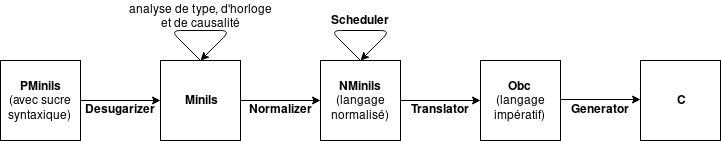
\includegraphics[width=.7\paperwidth]{assets/chain.png}
  \caption{Passes de compilation}
  \label{fig:passesCompil}
\end{figure}

\section{Extensions}

\subsection{Polymorphisme d'horloge}

La première (légère) extension réalisée est un ajout par rapport aux règles de typages données dans~\cite{Biernacki08}. En effet, les règles de typages d'horloge données par l'article exigent que toutes les flux d'entrées (et de sortie) d'une application soient sur la même horloge. On décide dans cette extension de relaxer cette contrainte, en introduisant une notion de ``polymorphisme'' d'horloge lors de l'appel à une node.

On va pour cela profiter de la syntaxe de l'appel de fonction dans notre langage, qui permet de préciser une expression de \texttt{every} pour tout appel de node. On infère l'horloge qui sera l'horloge de base de la node interne (celle sur laquelle celle-ci sera exécutée) en unifiant les horloges de retour attendues, avec les horloges de retour déclarées pour la node. On compose ensuite cette horloge de base avec les horloge des paramètres formels de la node, pour obtenir les horloges des paramètres passés, qu'on doit alors vérifier. Par exemple, le typage d'horloge des nodes suivantes est accepté.

\begin{lstlisting}
node test_op(b : bool) returns (z : int when True(b));
let
  z = 3 when True(b);
tel;

node test_app(b1 : bool; c1 : bool) returns (z : int when True(c1) when True(b1));
let
  z = test_op(b1 when True(c1));
tel;
\end{lstlisting}

\subsection{Automates}

\subsection{Interpreteur}
\label{interpreter}

\subsection{Vérification des phases de compilation}
\label{compilVerif}

\cite{Colaco05}

\section{Difficultés rencontrées}

\bibliography{biblio}{}
\bibliographystyle{unsrt}

\end{document}
